% Generated by paper/build_imt_parameter_figures.py; do not hand edit.
% Q1 grid SHA-256: 1a48a6f4d5a4c6c1449f35cd7e5584b7a14d4a08f8effc2c4508497e8ef20058
\begin{figure}[tb]
\centering
\begin{minipage}[t]{\linewidth}
\centering
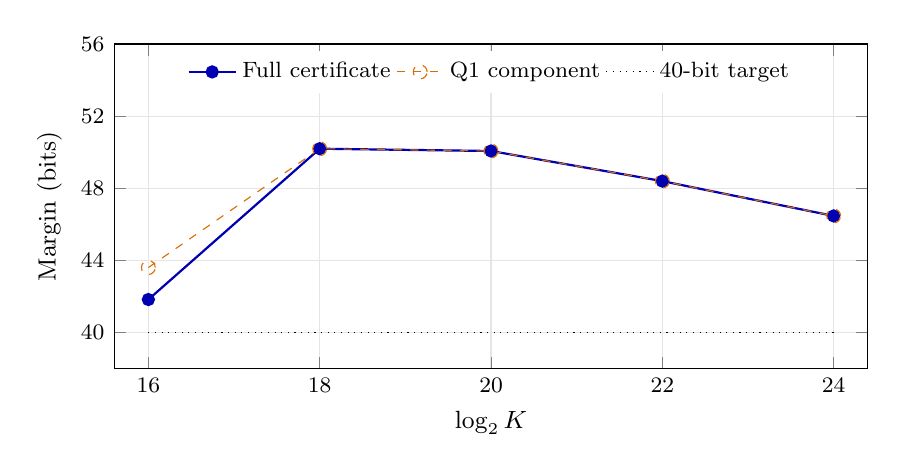
\begin{tikzpicture}
\begin{axis}[tick label style={font=\footnotesize},label style={font=\small},title style={font=\small},grid=major,grid style={black!10},legend style={font=\footnotesize,draw=none},width=.92\linewidth,height=5.7cm,xlabel={$\log_2 K$},ylabel={Margin (bits)},xmin=15.6,xmax=24.4,ymin=38,ymax=56,xtick={16,18,20,22,24},ytick={40,44,48,52,56},legend style={at={(.5,.98)},anchor=north,legend columns=3},]
\addplot[blue!70!black,thick,mark=*,mark size=2pt] coordinates {(16,41.8183267960) (18,50.1890763816) (20,50.0620882264) (22,48.3904916829) (24,46.4572549297)};
\addlegendentry{Full certificate}
\addplot[orange!85!black,dashed,mark=o,mark size=2.5pt] coordinates {(16,43.5928335021) (18,50.1891811139) (20,50.0622720959) (22,48.3904952900) (24,46.4572568186)};
\addlegendentry{Q1 component}
\addplot[black,dotted] coordinates {(16,40.0000000000) (24,40.0000000000)};
\addlegendentry{40-bit target}
\end{axis}
\end{tikzpicture}
\end{minipage}
\caption{Matched Q1 components and complete outward bounds for the selected
BCH-256, IMT $(128,19)$ construction. Both curves use exactly the same
maps and setup distribution. The four larger-length pairs nearly coincide.
Connecting segments do not certify intermediate lengths.}
\label{fig:finite-bch-curve}
\end{figure}
